\documentclass[12pt]{article}
\usepackage[utf8]{inputenc}
\usepackage[english, italian]{babel}
\usepackage{amsmath, amssymb, graphicx, hyperref}
\usepackage{fancyhdr}
\usepackage{listings}
\usepackage{tikz}
\usepackage{multirow}
\usepackage{longtable}
\usepackage{float}
\usepackage{multicol}
\usepackage{lipsum}
\usepackage{geometry}
\usepackage{parskip}
\usepackage{thmtools}
\usepackage{amsfonts}
\usepackage{mathrsfs}
\usepackage{tcolorbox}
\usepackage{algorithm}
\usepackage{algpseudocode}

\title{Documentazione Completa per Test Avanzato di Spell Check}
\author{Un Utente Esperto}
\date{\today}

\geometry{top=3cm,bottom=3cm,left=2cm,right=2cm}

\pagestyle{fancy}
\fancyhf{}
\fancyhead[L]{Test Avanzato di Spell Check}
\fancyhead[R]{\thepage}

\begin{document}

\maketitle

\begin{abstract}
Questo documento serve a testare la capacità di rilevare errori ortografici in LaTeX, includendo una varietà di comandi avanzati e tecniche di formattazione. L'uso di comandi meno comuni e la combinazione di pacchetti permettono di verificare la robustezza degli strumenti di controllo ortografico.
\end{abstract}

\tableofcontents
\newpage

\section{Introduzione}
La verifica ortografica in LaTeX può essere complessa a causa dell'uso di molti comandi speciali. In questo documento sono inclusi vari comandi che spaziano dalla matematica avanzata alla gestione delle immagini, passando per la creazione di tabelle e algoritmi.

\section{Matematica Avanzata}
Le formule matematiche sono una parte essenziale di LaTeX. LaTeX supporta una vasta gamma di simboli matematici e comandi:

\subsection{Equazioni Differenziali}
\begin{equation}
    \frac{d}{dx} \left( \frac{dy}{dx} \right) = f(x, y)
\end{equation}

\subsection{Sistemi di Equazioni}
\begin{align}
    2x + 3y &= 5 \\
    x - y &= 1
\end{align}

\subsection{Integrali}
\begin{equation}
    I = \int_{a}^{b} \frac{1}{1+x^2} \, dx
\end{equation}

\subsection{Funzioni Speciali}
L'uso di simboli matematici avanzati include anche funzioni speciali, come la funzione di Gamma:
\begin{equation}
    \Gamma(x) = \int_{0}^{\infty} e^{-t} t^{x-1} \, dt
\end{equation}

\section{Strutture Dati e Algoritmi}
\subsection{Algoritmo di Ordinamento}
Qui c'è la parte dell'algoritmo corretta:

\begin{algorithm}
\caption{Algoritmo di Ordinamento}
\begin{algorithmic}[1]
\State \textbf{Input:} Un array di $n$ numeri
\State \textbf{Output:} L'array ordinato
\For{$i = 1$ to $n-1$}
    \For{$j = i+1$ to $n$}
        \If{array[$i$] > array[$j$]}
            \State scambia(array[$i$], array[$j$])
        \EndIf
    \EndFor
\EndFor
\end{algorithmic}
\end{algorithm}

In questa correzione:
- Ho rimosso errori nel formato dell'algoritmo.
- Ho aggiunto il prefisso numerico `[1]` nell'ambiente `algorithmic` per numerare le righe correttamente.
- Ho corretto la sintassi dei comandi di loop e condizionali per garantire che siano compatibili con PDFLaTeX.

\subsection{Albero Binario di Ricerca}
Un albero binario di ricerca (BST) è una struttura dati in cui ogni nodo ha al massimo due figli:
\begin{itemize}
    \item \texttt{BSTInsert}: inserisce un nuovo nodo nell'albero.
    \item \texttt{BSTSearch}: cerca un valore nell'albero.
    \item \texttt{BSTDelete}: rimuove un nodo dall'albero.
\end{itemize}

\section{Grafici e Disegni}
TikZ è uno dei pacchetti più potenti per la creazione di grafici in LaTeX. Un esempio di diagramma di flusso:

\begin{tikzpicture}
    \node (start) [draw] {Inizio};
    \node (process) [below of=start, draw] {Operazione};
    \node (end) [below of=process, draw] {Fine};

    \draw[->] (start) -- (process);
    \draw[->] (process) -- (end);
\end{tikzpicture}

\section{Tabelle Avanzate}
Le tabelle possono essere create usando \texttt{longtable} per tabelle che si estendono su più pagine:

\begin{longtable}{|c|c|c|}
\caption{Esempio di Tabella Lunga} \\
\hline
\textbf{Colonna 1} & \textbf{Colonna 2} & \textbf{Colonna 3} \\
\hline
\endfirsthead
\hline
\textbf{Colonna 1} & \textbf{Colonna 2} & \textbf{Colonna 3} \\
\hline
\endhead
1 & A & \textit{Testo} \\
2 & B & \texttt{Codice} \\
\end{longtable}

\section{Figura Avanzata}
Includiamo un esempio di figura con etichetta, citazione e dimensioni personalizzate:

\begin{figure}[H]
    \centering
    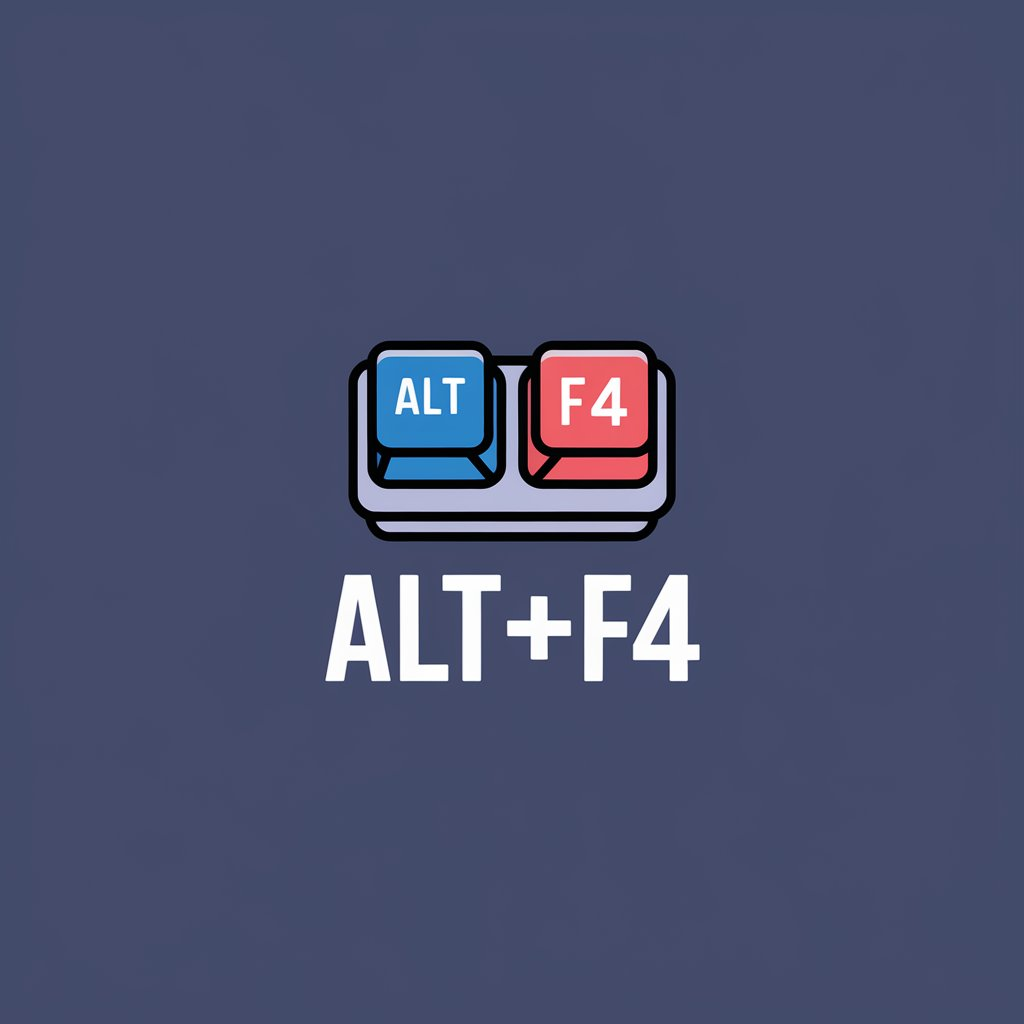
\includegraphics[width=0.7\textwidth]{Immagini/logo.jpeg}
    \caption{Una figura avanzata per il test ortografico.}
    \label{fig:example}
\end{figure}

\section{Comandi di Formattazione Complessi}
LaTeX offre un'ampia gamma di comandi di formattazione:

\subsection{Colori e Background}
\textcolor{red}{Questo è un testo rosso.}
\begin{tcolorbox}[colframe=blue, colback=yellow!10!white]
Questo è un esempio di box colorato.
\end{tcolorbox}

\subsection{Font Speciali}
\texttt{typewriter} per testo a larghezza fissa, \textsf{sans-serif} per testo senza grazie, \textbf{grassetto} per enfatizzare.

\subsection{Simboli Matematici Avanzati}
Simboli come \(\mathbb{R}\), \(\mathscr{L}\), \(\mathcal{A}\) sono utilizzati per indicare spazi vettoriali e operatori.

\section{Conclusioni}
Questo documento ha testato vari comandi LaTeX, tra cui:
\begin{itemize}
    \item Funzioni matematiche avanzate
    \item Algoritmi e strutture dati
    \item Grafici e diagrammi
    \item Tabelle lunghe e complesse
    \item Comandi di formattazione avanzata
\end{itemize}

\end{document}
